\newpage
\section{Theoretical framework}
I start by setting out the canonical model of Mace (1991)  \nocite{mace1991full} to show how aggregate shocks impact individual consumption. This is a simple framework which I use to show how individual consumption varies with aggregate shocks. I then add an extension to this model by incorporating mobile money services as a flow of remittances to households. This allows me to determine three cases of the impact of aggregate shocks on consumption with and without mobile money services and with different degrees of village sharing of remittances.   

\subsection{Aggregate shocks}

As in the Mace model, I consider a village of risk-averse utility maximising households indexed by $j=1 \ldots J$. There are T periods and village states of nature $s_{\tau t}, \tau=1 \ldots S$. There is a probability $\pi(s_{\tau t})$ that state $\tau$ occurs in period $t$ such that $\sum_{\tau=1}^{S} \pi(s_{\tau t})=1$.  Each household has utility $U(C^j(s_{\tau t}),h^j(s_{\tau t}))$ where $C^j_t(s_{\tau t})$ is consumption and $h^j(s_{\tau t})$ is a preference shock representing changes in taste for consumption and both can be functions of the state of the world over time. I assume each household receives an exogenous amount of the consumption good $y_t^j(s_{\tau t})$ which is visible to everyone in the community. Households have no access to savings or credit. 

Mace showed (see Appendix) that for the Pareto efficient outcome to be achieved:
\begin{equation} \label{eq: FOC1}
\frac{U'(C^i_t(s_{\tau t}))}{U'(C^j_t(s_{\tau t}))}=\frac{\lambda^j}{\lambda^i} \qquad \forall i, j, \tau, t
\end{equation}
where $\lambda^i$ is the welfare weight for household $i$. This condition says that the weighted marginal utilities are equated across households so that any household's consumption is a monotonically increasing function of average village consumption. 

I consider Mace's second class of utility functions, the power utility functions, that exhibit constant relative risk aversion: 
\begin{equation}
U(c,h)= \exp{\sigma h^j_t}\frac{1}{\sigma}(C^j_t)^{\sigma}
\end{equation}
Applying this utility functional form to the first order condition \eqref{eq: FOC1} aggregating over $J$ households and taking logarithms gives the consumption for a household as:
\begin{equation} \label{eq: consumption}
\ln C_t^j(s_{\tau t}) = \ln C^a_t(s_{\tau t}) + \frac{1}{1-\sigma}(\ln \lambda^i- \lambda^a) + \frac{\sigma}{1-\sigma}(h^i- h^a_t(s_{\tau t}))
\end{equation}
where
\[
C_t^a=\frac{1}{J} \sum_{j=1}^J \ln C_t^j \qquad \lambda^a=\frac{1}{J} \sum_{j=1}^J \ln \lambda^j \qquad  h^a_t=\frac{1}{J} \sum_{j=1}^J \ln h_t^j
\]
Mace showed that household consumption depends on aggregate consumption in the village plus a time invariant household fixed effect $\lambda$, which depends on the relative weight in the Pareto optimum allocation, and preference shifters. Individual shocks are perfectly insured at the village level and do not affect household consumption. As mentioned in the initial assumptions, households have no savings in this model. This is to allow deviations from perfect risk sharing to be examined. While in reality households use other methods to smooth their consumption such as savings and credit, these can be controlled for in the empirical specification. 

I am interested in aggregate shocks, therefore I decompose the individual endowment of each household into its deterministic income, aggregate shock and idiosyncratic components assuming these are independent of each other:
Household $j$ receives an exogenous endowment of the consumption good $y^j_t(s_{\tau t})$ which is visible to everyone in the village. This can be decomposed into the deterministic and stochastic components: 
\begin{equation} \label{eq: endow}
y^j_t(s_{\tau t}) = \bar{y}^j_t + \eta_t^j(s_{\tau t}) + \epsilon_t^j(s_{\tau t})
\end{equation}
where $\bar{y}^j_t$ is the deterministic portion of output, $\eta_t^j(s_{\tau t})$ is an aggregate shock to household $j$'s endowment (which may still differ across households) and $\epsilon_t^j(s_{\tau t})$ is the idiosyncratic shock experiences by household $j$ only. When equation \eqref{eq: endow} is aggregated across $J$ households the aggregate endowment is given by:
\begin{equation} \label{eq:agg endow1}
y^a_t(s_{\tau t}) = \bar{y}^a_t + \eta_t^a(s_{\tau t})
\end{equation}
where 
\[
y^a_t(s_{\tau t})= \frac{1}{J}\sum_{j=1}^Jy^j_t(s_{\tau t}) \qquad \bar{y}^a_t= \frac{1}{J}\sum_{j=1}^J \bar{y}^j_t \qquad  \eta^a_t=\frac{1}{J}\sum_{j=1}^J\eta_t^j(s_{\tau t}) \qquad \sum_{j=1}^J \epsilon_t^j(s_{\tau t})=0
\]
Idiosyncratic shocks balance out within the village as J approaches infinity. Aggregate uncertainty means $\eta_t^a(s_{\tau t}) \neq 0$ for at least one event for all $t$. The aggregate resource constraint says that $C^a_t=y^a_t$ therefore I can substitute \eqref{eq:agg endow1} into equation \eqref{eq: consumption}. 
\begin{equation} \label{eq: agg shock}
\ln C_t^j(s_{\tau t}) = \ln (\bar{y}^a_t + \eta_t^a(s_{\tau t})) + \frac{1}{1-\sigma}(\ln \lambda^i- \lambda^a) + \frac{\sigma}{1-\sigma}(h^i- h^a_t(s_{\tau t}))
\end{equation}
Household consumption depends on the deterministic component of village consumption $\bar{y}$, an aggregate shock $\eta$, a household fixed effect and preference shifts. Idiosyncratic shocks are perfectly insured by the village as $J \rightarrow \infty$. However, for a village in which all households experience the same aggregate shock at once, consumption will fall. 

\subsection{Mobile money}
The above section showed how individual consumption depends on aggregate shocks. I will now combine this with mobile money services and look at how mobile money allows remittances from someone outside the village to respond to the aggregate shock. I will consider mobile money users, non-users in villages with mobile money and non-users in villages without mobile money. 

I consider an economy in which households can only share risk with each other when there is a social tie between them. Households have social ties both with households within their own village but also with households outside their village, for example if a member of their household leaves the village to work in another village or the city (a migrant). Having links with people outside the village in far away locations increases the diversification of income streams across the risk sharing network. The set of social networks is taken as given. With no constraints on commitment or enforcement and the network connected (so that everyone is linked up in the network), risk sharing will be efficient. However, if networks are closed such that different networks are not linked then exchange is limited to members of one's own network. 

I assume that transfers can only take place via mobile money payments so that only households that use mobile money can receive remittances after an aggregate shock. Aggregate shocks are assumed to not be perfectly correlated across locations so that reciprocal transfers are possible between different locations undergoing shocks at different times. If there is at least one household in a village that receives a transfer via mobile money, this will be shared with everyone else in the village due to the perfect risk sharing assumption discussed above. 
Members of a village who don't use mobile money themselves but with at least one mobile money user can receive transfers from the mobile money using household. In a perfect risk sharing world, a recipient of remittances is assumed to share these perfectly with other members of their risk sharing network. Remittances therefore provide insurance to the entire village and dampen the negative effect of the aggregate shock.

As an example, suppose there are three households, $A$, $B$ and $C$.  Households $B$ and $C$ both reside in the same village, but $A$ is in another village far away. Household $B$ is connected to both households $A$ and $C$ in a risk-sharing network and so able to facilitate exchange with both of them. If $B$ and $C$ experience an aggregate shock in their village, $A$ can send transfers to them through $B$ via mobile money. $B$ will then share any remittances with $C$ and so dampen the impact of the aggregate shock for both. 

Expanding this model to many households within each village, mobile money use can be seen to connect the village risk sharing network to households outside the village. The more mobile money users there are in a village, and the more connections these households have to households in other villages, the more smoothing there will be of consumption after an aggregate shock. I assume that the sender of remittances has past information about the size of losses after aggregate shocks and so sends an amount equal to the average of these losses. Assuming the majority of remittance senders were once living in the household as children, they should have an idea of how large losses would be in the event of a shock and send an amount expected to cover this.  Households who don't use mobile money themselves can only receive transfers from the households within their village that do use mobile money. For example, the amount of transfers that household $C$ receives will be increasing in the proportion of other households in the village who use mobile money, assuming they are linked to different migrants who send them remittance. 

I can also use this as a test of the degree that remittances are shared perfectly within a village. If the recipient of the mobile money does not share the remittance with other members of the village, then that household will better smooth its income after the aggregate shock than other households in the village, and this can be tested in the data. Possible reasons for not sharing the remittance are being able to hide the remittance from other members of the village or because the household with a migrant member chooses to insure itself through that network instead of through the village risk sharing network. 

If there are two other households, $D$ and $E$, who are located in different villages but not connected to each other via mobile money, when $E$'s village suffers from an aggregate shock, $D$'s village will be unable to insure it. 

This gives 3 cases for the impact of an exogenous rainfall shock which I will formalise as: 

\textbf{Case 1: No mobile money use}. Non-users in villages without mobile money will experience the full negative impact of the aggregate shock $\eta_t^a(s_{\tau t})$  on each household's consumption as in equation \eqref{eq: agg shock}. 

Case 1 (no mobile money use) is shown in Figure \ref{fig: no link}. 
\begin{figure}[h]
    \centering
    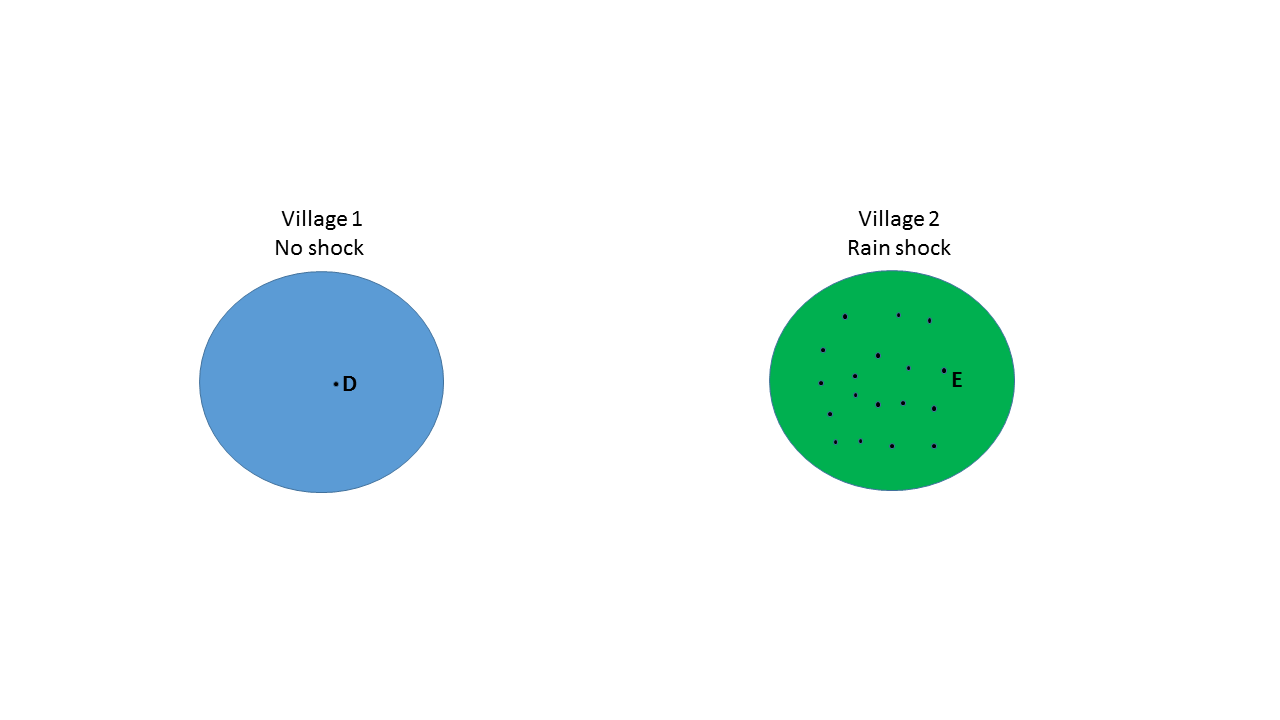
\includegraphics[width=17cm,trim=0cm 4cm 0cm 4cm,clip=true, keepaspectratio]{Slide1new}
\caption{Case 1: No mobile money use}
    \label{fig: no link}
\end{figure}
There are two villages with a migrant in village 1, D, and a home network Village 2 which experiences a rain shock. However without any links to D in village 1, the households of village 2 will experience a drop in consumption since they are unable to insure themselves against the aggregate shock.

\textbf{Case 2: Perfect village sharing}. In villages with mobile money, I assume $M$ users of mobile money and $N$ non-users such that $N+M=J$. Users of mobile money receive a transfer $t^m$ which is insufficient to cover the impact of the aggregate shock for the entire village, $t^m<J\eta_t^a(s_{\tau t})$ but can cover the aggregate shock for one household $t^m=\eta_t^a(s_{\tau t})$. With $M$ mobile-money-using households each receiving a transfer $t^m$ and shared between $J$ households, each household receives $\frac{M}{J}t^m$. 

It can be seen that all households are partially insured against the aggregate shock by $\frac{M}{J} t^m<\eta_t^a(s_{\tau t})$ which increases proportionately to the number of mobile-money-using households in the community such that if all households use mobile money and receive remittances the aggregate shock would be completely insured against. All households will get consumption of:
\begin{equation} \label{eq: perfect sharing}
\ln C_t^j(s_{\tau t}) = \ln (\bar{y}^a_t + \eta_t^a(s_{\tau t}) + \frac{M}{J}t^m) + \frac{1}{1-\sigma}(\ln \lambda^i- \lambda^a) + \frac{\sigma}{1-\sigma}(h^i- h^a_t(s_{\tau t}))
\end{equation}

Case 2 is shown in Figure \ref{fig:link}. 
\begin{figure}[p]
    \centering
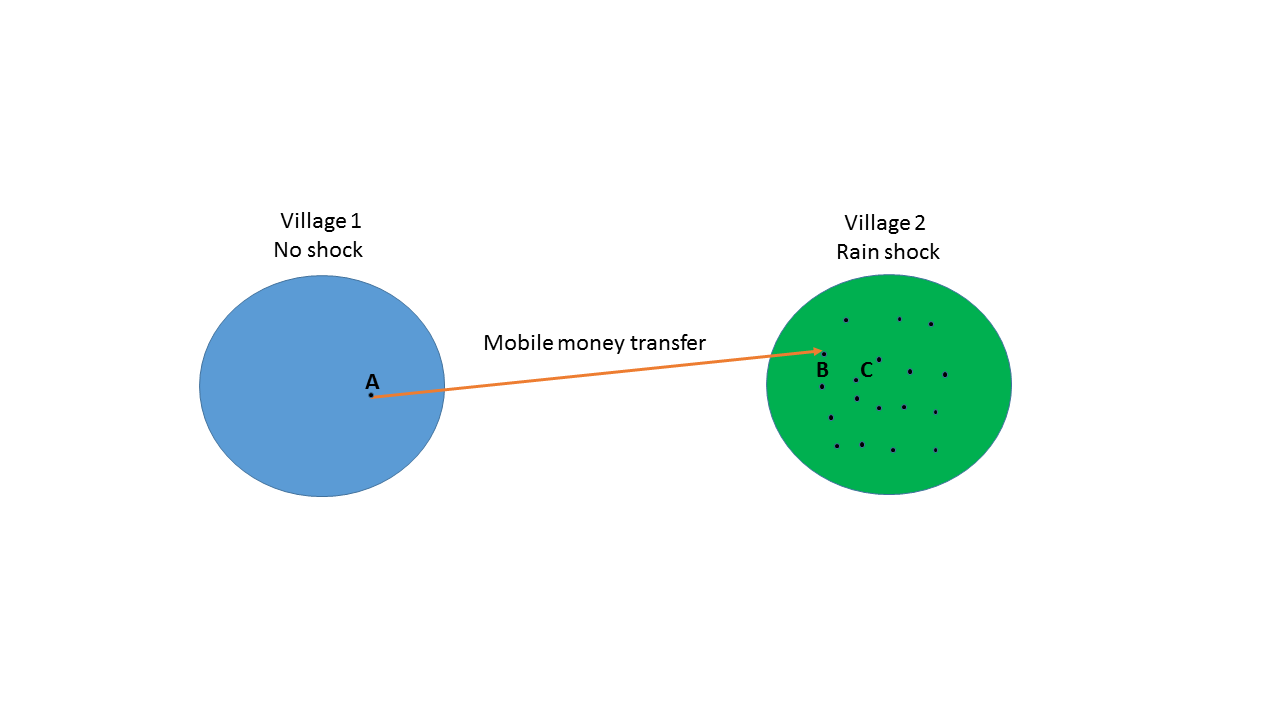
\includegraphics[width=17cm,trim=0cm 4cm 0cm 4cm,clip=true, keepaspectratio]{Slide2.PNG} 
\caption{Case 2: mobile money use and perfect risk sharing in villages}
    \label{fig:link}
\end{figure}
The migrant worker in village 1, $A$, is linked via mobile money to household $B$ in village 2. When village 2 experiences a rainfall shock, household $A$ sends money to household B who then shares this with all the other households in the village, such as $C$. Hence there are benefits in mobile money use to the rest of the community. Every household experiences a small drop in consumption due to the aggregate shock since $A$ cannot insure the entirety of village 2. The amount of insurance will be increasing in the number of distinct links to migrants in outside villages. 

\textbf{Case 3: The mobile-money-using household does not share the remittance with other households in the village.}
The mobile money using household receives the transfer $t^m$ and does not share this with the rest of the community,  but uses it itself to smooth the aggregate shock. Whatever the reason for the household not sharing the remittances, if remittances are not shared there will be no consumption smoothing benefit from mobile money users to other members of the community.  Mobile-money-using households will get consumption of:
\begin{equation} \label{eq: MM users}
\ln C_t^j(s_{\tau t}) = \ln (\bar{y}^a_t + \eta_t^a(s_{\tau t}) + t^m) + \frac{1}{1-\sigma}(\ln \lambda^i- \lambda^a) + \frac{\sigma}{1-\sigma}(h^i- h^a_t(s_{\tau t}))
\end{equation}
where the transfer $t^m$ exactly counters the negative aggregate shock $\eta^a$.

Case 3 is shown in Figure \ref{fig:link2}.
\begin{figure}[p]
    \centering
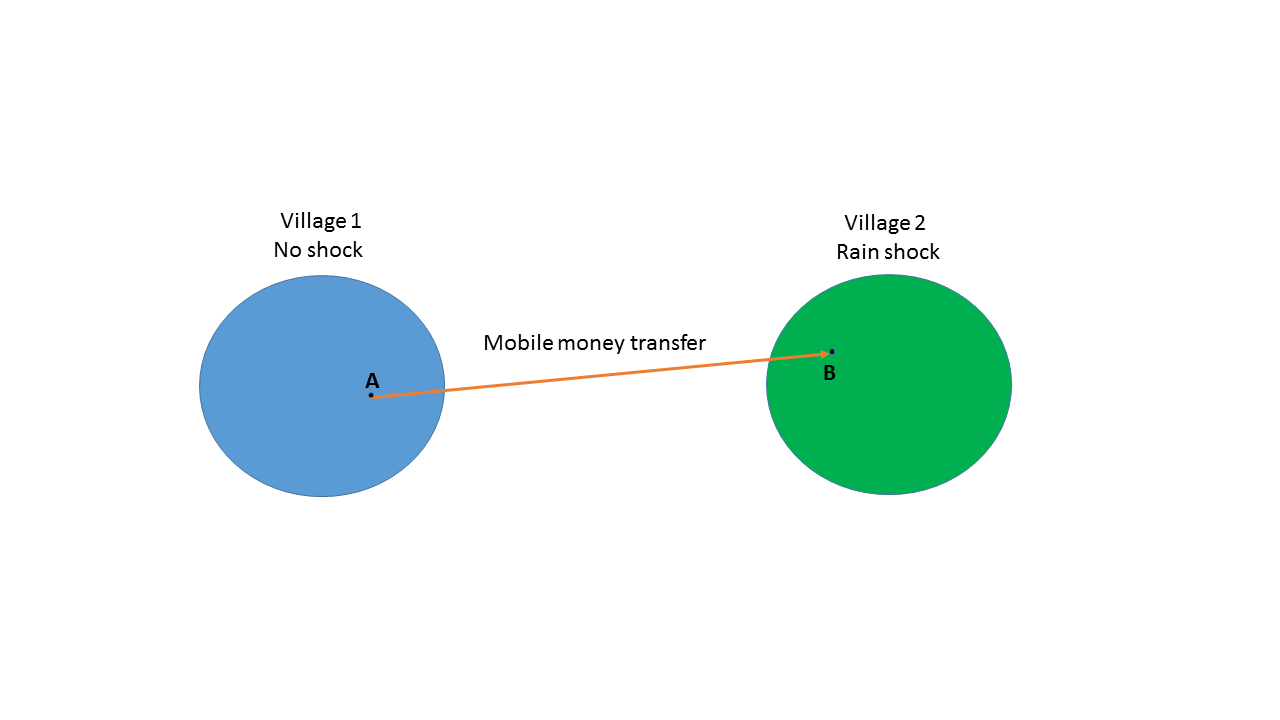
\includegraphics[width=17cm,trim=0cm 4cm 0cm 4cm,clip=true, keepaspectratio]{Slide3new} 
\caption{Case 3: villages with mobile money where the mobile money recipient does not share the remittance with the other village households }
    \label{fig:link2}
\end{figure}
When village 2 experiences a rainfall shock, household $A$ sends money to household $B$, compensating the household for any drop in consumption due to the aggregate shock. $B$ does not share this with other households in the village. Other households in village 2, will therefore still suffer a drop in consumption due to the aggregate shock.



